\documentclass[border=10pt]{standalone}
\usepackage{mathptmx}
\usepackage{amsmath,bm}
\usepackage{tikz}
\usetikzlibrary{arrows.meta,positioning,fit,calc,backgrounds}
\definecolor{gdark}{HTML}{5E7B5F}
\definecolor{glight}{HTML}{E6E9E4}
\definecolor{gbord}{HTML}{4A634B}
\definecolor{rloss}{HTML}{A8323E}
\definecolor{rsoft}{HTML}{F3DCDD}
\definecolor{note}{HTML}{F4F1E8}
\tikzset{
  dk/.style={draw=gbord,fill=gdark,text=white,rounded corners=3pt,align=center,font=\small,minimum height=12mm,minimum width=30mm,inner sep=5pt},
  lt/.style={draw=gray!60,fill=glight,text=black,rounded corners=3pt,align=center,font=\small,minimum height=12mm,minimum width=30mm,inner sep=5pt},
  ls/.style={draw=rloss,fill=rsoft,text=black,rounded corners=3pt,align=center,font=\small,minimum height=12mm,minimum width=30mm,inner sep=5pt,line width=0.8pt},
  nt/.style={draw=gray!50,fill=note,text=black!80,rounded corners=3pt,align=left,font=\footnotesize,inner sep=6pt},
  ar/.style={-{Stealth[length=2.6mm]},line width=0.8pt,draw=black!75},
  ard/.style={-{Stealth[length=2.6mm]},line width=0.8pt,draw=rloss,dashed},
  lb/.style={font=\footnotesize\itshape,text=black!70,align=center},
  frame/.style={draw=gbord,rounded corners=6pt,dashed,line width=0.7pt,inner sep=8pt},
  ttl/.style={font=\large\bfseries,text=black}
}
\newcommand{\x}{\bm{x}}

\begin{document}
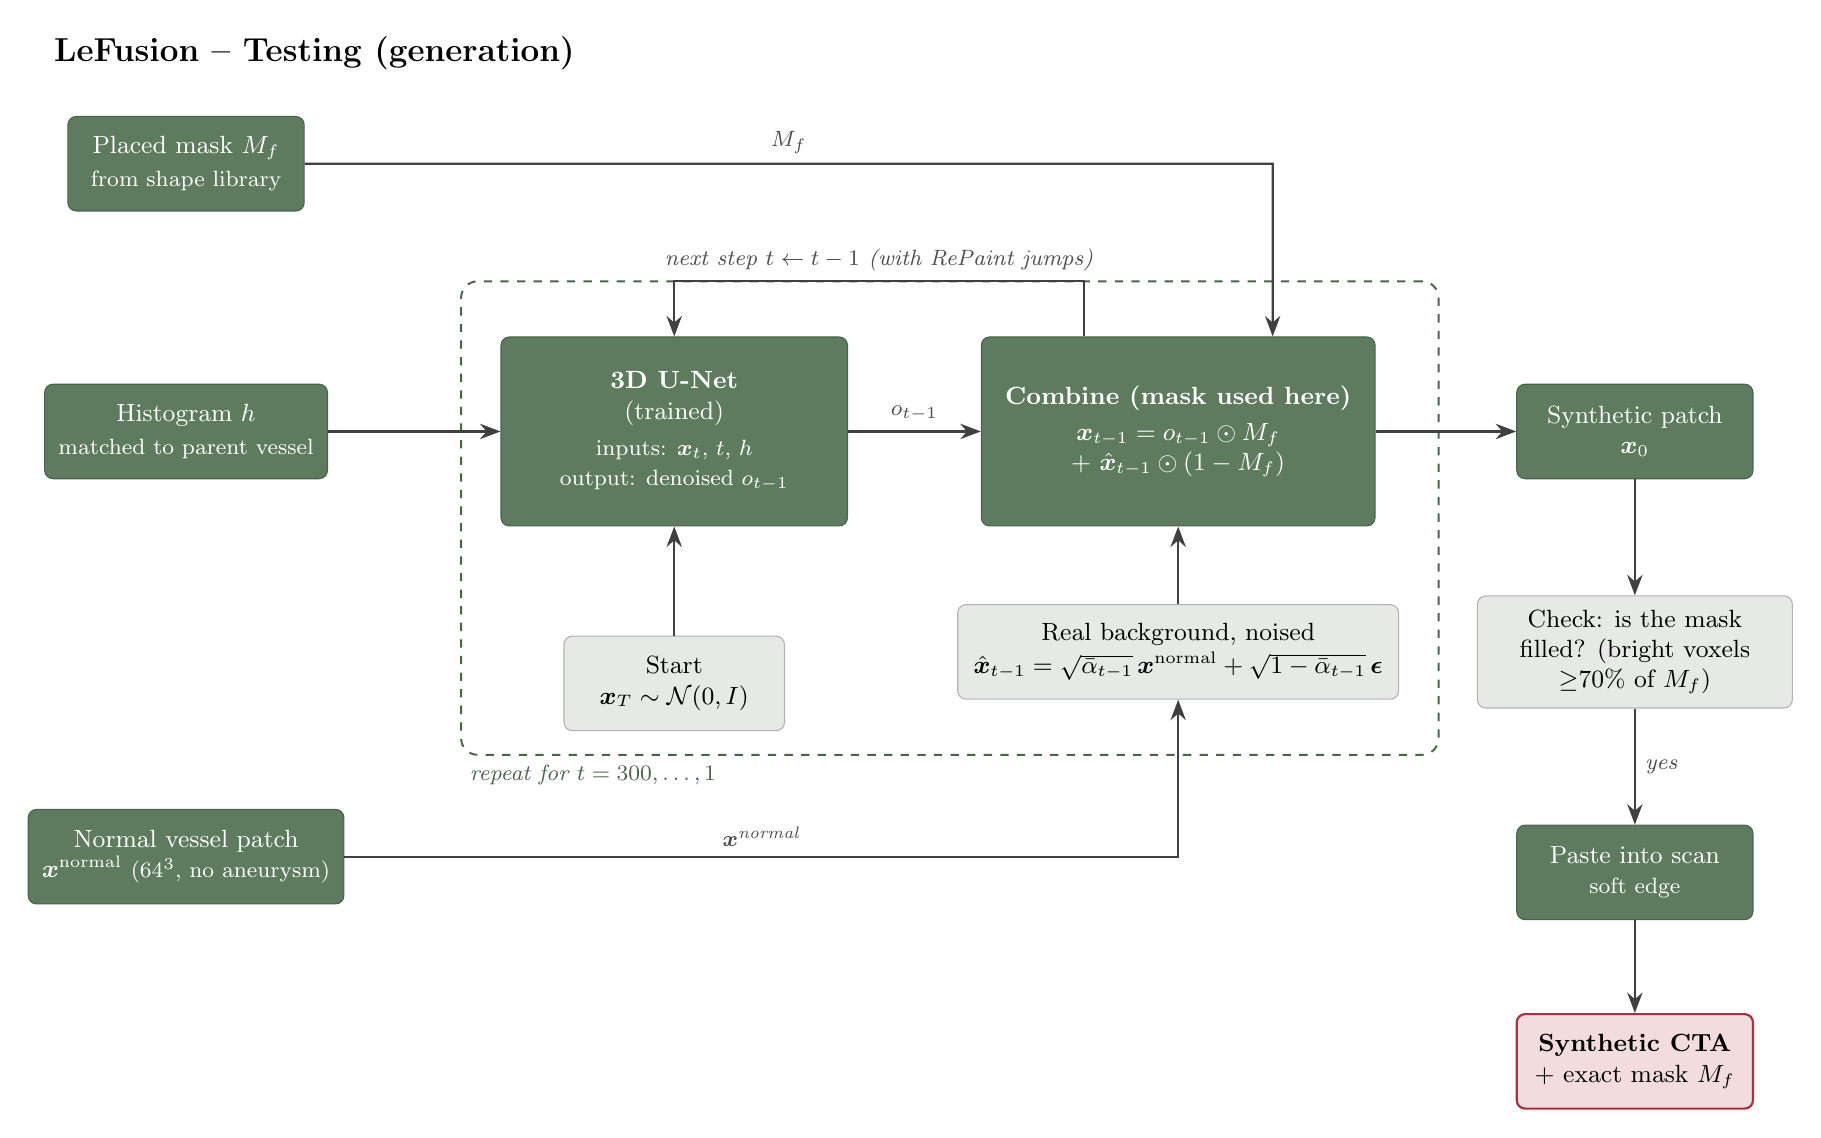
\begin{tikzpicture}[x=1mm,y=1mm]
\node[ttl, anchor=west] at (-18,36) {LeFusion -- Testing (generation)};
% inputs
\node[dk] (mf) at (0,22) {Placed mask $M_f$\\[1pt]\footnotesize from shape library};
\node[dk] (h) at (0,-12) {Histogram $h$\\[1pt]\footnotesize matched to parent vessel};
\node[dk] (vp) at (0,-66) {Normal vessel patch\\$\x^{\text{normal}}$ \footnotesize ($64^3$, no aneurysm)};
% loop
\node[dk, minimum width=44mm, minimum height=24mm] (u) at (62,-12) {\textbf{3D U-Net}\\(trained)\\[2pt]\footnotesize inputs: $\x_t$, $t$, $h$\\\footnotesize output: denoised $o_{t-1}$};
\node[dk, minimum width=50mm, minimum height=24mm] (cb) at (126,-12) {\textbf{Combine (mask used here)}\\[2pt]$\x_{t-1}=o_{t-1}\odot M_f$\\$+\ \hat\x_{t-1}\odot(1-M_f)$};
\node[lt, minimum width=56mm] (bg) at (126,-40) {Real background, noised\\[1pt]$\hat\x_{t-1}=\sqrt{\bar\alpha_{t-1}}\,\x^{\text{normal}}+\sqrt{1-\bar\alpha_{t-1}}\,\bm\epsilon$};
\node[lt, minimum width=28mm] (xT) at (62,-44) {Start\\$\x_T\sim\mathcal N(0,I)$};
\draw[ar] (u)--node[lb,above]{$o_{t-1}$}(cb);
\draw[ar] (bg)--(cb);
\draw[ar] (xT)--(u);
\draw[ar] ([xshift=-12mm]cb.north) -- ++(0,7) -| node[lb,pos=0.25,above]{next step $t\leftarrow t-1$ (with RePaint jumps)} (u.north);
\begin{scope}[on background layer]\node[frame, fit=(u)(cb)(bg)(xT), inner sep=5mm, yshift=2mm] (loop) {};\end{scope}
\node[lb, anchor=north west, text=gbord] at (loop.south west) {repeat for $t=300,\dots,1$};
% feeds
\draw[ar] (h.east) -- (h.east -| u.west);
\draw[ar] (mf.east) -- node[lb,above,pos=0.5]{$M_f$} (138,22) -- ([xshift=12mm]cb.north);
\draw[ar] (vp.east) -- node[lb,above,pos=0.5]{$\x^{\text{normal}}$} (126,-66) -- (bg.south);
% output
\node[dk] (o1) at (184,-12) {Synthetic patch\\$\x_0$};
\node[lt, minimum width=40mm] (qc) at (184,-40) {Check: is the mask\\filled? (bright voxels\\$\geq$70\% of $M_f$)};
\node[dk] (o2) at (184,-68) {Paste into scan\\\footnotesize soft edge};
\node[ls] (o3) at (184,-92) {\textbf{Synthetic CTA}\\+ exact mask $M_f$};
\draw[ar] (cb.east) -- (o1.west); \draw[ar] (o1)--(qc); \draw[ar] (qc)--node[lb,right]{yes}(o2); \draw[ar] (o2)--(o3);
\end{tikzpicture}
\end{document}
